\begin{minipage}[t]{504pt}
\begin{minipage}[t]{350pt}
\setlength{\parindent}{\myindent}
\setlength{\parskip}{\myparskip}

 \vspace*{-8pt}


 \section{Past research}
 As part of my Information Technology major field, I had the opportunity to participate in 
 the Data Driven Engineering I/II course series by Dr. Cihan Ates, where I obtained a solid foundation in machine learning 
 and optimization. With my first machine learning research project "Energy Consumption Prediction at High Granularity" 
 I competed at the lecture accompanying project contest, where I placed in the top three . 
 \color{yellow}I gained valuable experience in the practical 
 application of classical regression methods, such as Linear regression, Support Vector Regression and Random Forest models. 
 In a second step I compared the performance of the
  classical methods with Recurrent Neural Networks and LSTM based neural network models. \color{black} \todo{make broader and less}
  In Data Driven Engineering II, my team and I worked on 
  particle velocity and uncertainty estimation using convolutional autoencoders based on a variance attenuation loss.
The excellent course in Machine Vision by Dr. Martin Lauer inspired me to focus more on perception and in particular object detection.

This led to my master's thesis titled "Masked Autoencoding as Pre-Training for Traffic Participant Detection," 
reviewed by Prof. Dr.-Ing. Christoph Stiller.
The goal of the thesis was to investigate self-supervised learning as a pretext task for downstream 2D and 3D object detection in the context 
of autonomous driving. For pretraining Masked Image Modeling in particular the popular Masked Autoencoding \cite{mae} technique was used. To achieve real-time performance within a flexible detection framework we chose CenterNet. It reframes 
object detection as a keypoint estimation task and additionally regress bounding box parameters from the predicted keypoints.
By performing 2D object detection on monocular images, 3D object detection on monocular images, and 3D object detection on bird's eye view
representations of the  lidar point cloud I was able to get an overview of the object detection field.
First we benchmarked the detector on KITTI using a ResNet backbone. After replacing the ResNet with a vision transformer we met 
the practical challenge of small dataset size, large image size, and model size when training a vision transformer with little 
inductive biases compared to CNN-based models.
While I saw decent results when using a pretrained vision transformer in the detectron-2 framework,
training a vision transformer from scratch on KITTI is not practical.
To mitigate these challenges we focussed on the larger Waymo Open Perception dataset using 
bird's eye view representations of the lidar point cloud. Further we investigated the impact of other vision transformers and found 
the hierarchical vision transformer Hiera \cite{hiera}. It comes with inductive biases like local attention in early layers and 
token pooling. Through the clever application of mask units Hiera allows for 
the use of Masked Autoencoding (MAE) as a pretext task. In \autoref{fig:mae_img} a exemplary MAE reconstruction of a 
bird's eye view point cloud representation
on the Waymo Open Perception dataset is shown. We showed that the 
MAE pretext task is beneficial for the downstream task of 3D object detection evaluated on the Waymo Open Perception validation set. 
regarding augmentation our findings align with 
prior research namely that pointcloud rotation augmentation increases the performance and mirror augmentation decreases the performance.

I continued my research at the Research Center for Information Technology (FZI), where I designed data and training pipelines 
to incorporate video sequence input as well as multimodal inputs to the Hiera model. The multimodal approach to fuse bird's eye view and 
spherical view of the lidar point cloud as shown in \autoref{fig:fusion} by jointly masking 
and reconstructing the embeddings of the two views. For that I designed separate encoders for the modalities 
similar to the \cite{multimae}. During MAE pretraining both modalities are reconstructed and during downstream 3D object detection
only the bird's eye view was used for the detection task. Ultimately we confirmed that the MAE task is beneficial 
for the downstream task of 3D object detection. Furthermore MAE can be used to fuse multimodal inputs in a self supervised way.
Finally by benchmarking against a ResNet backbone we showed that in the low data regime CNN-based architectures 
are still highly competitive in object detection.
The opportunity to utilize large public like Waymo Open Perception in addition 
 to training on the Jülich Supercomputing Centre, has enhanced my professional approach to machine learning. 
In a second project at FZI I processed accumulated point clouds and annotations in KITTI-360 
 towards a format suitable for frame by frame object detection similar to the KITTI dataset. The project shows
 that a theoretically optimal frame by frame object detector still needs optimal dissection and 
 accumulation of the point clouds and annotations to perform well on the KITTI-360 object detection benchmark.

 
\vspace*{-6pt}

\end{minipage}
\hspace{13pt}\begin{minipage}[t]{140pt}
\begin{figure}[H]
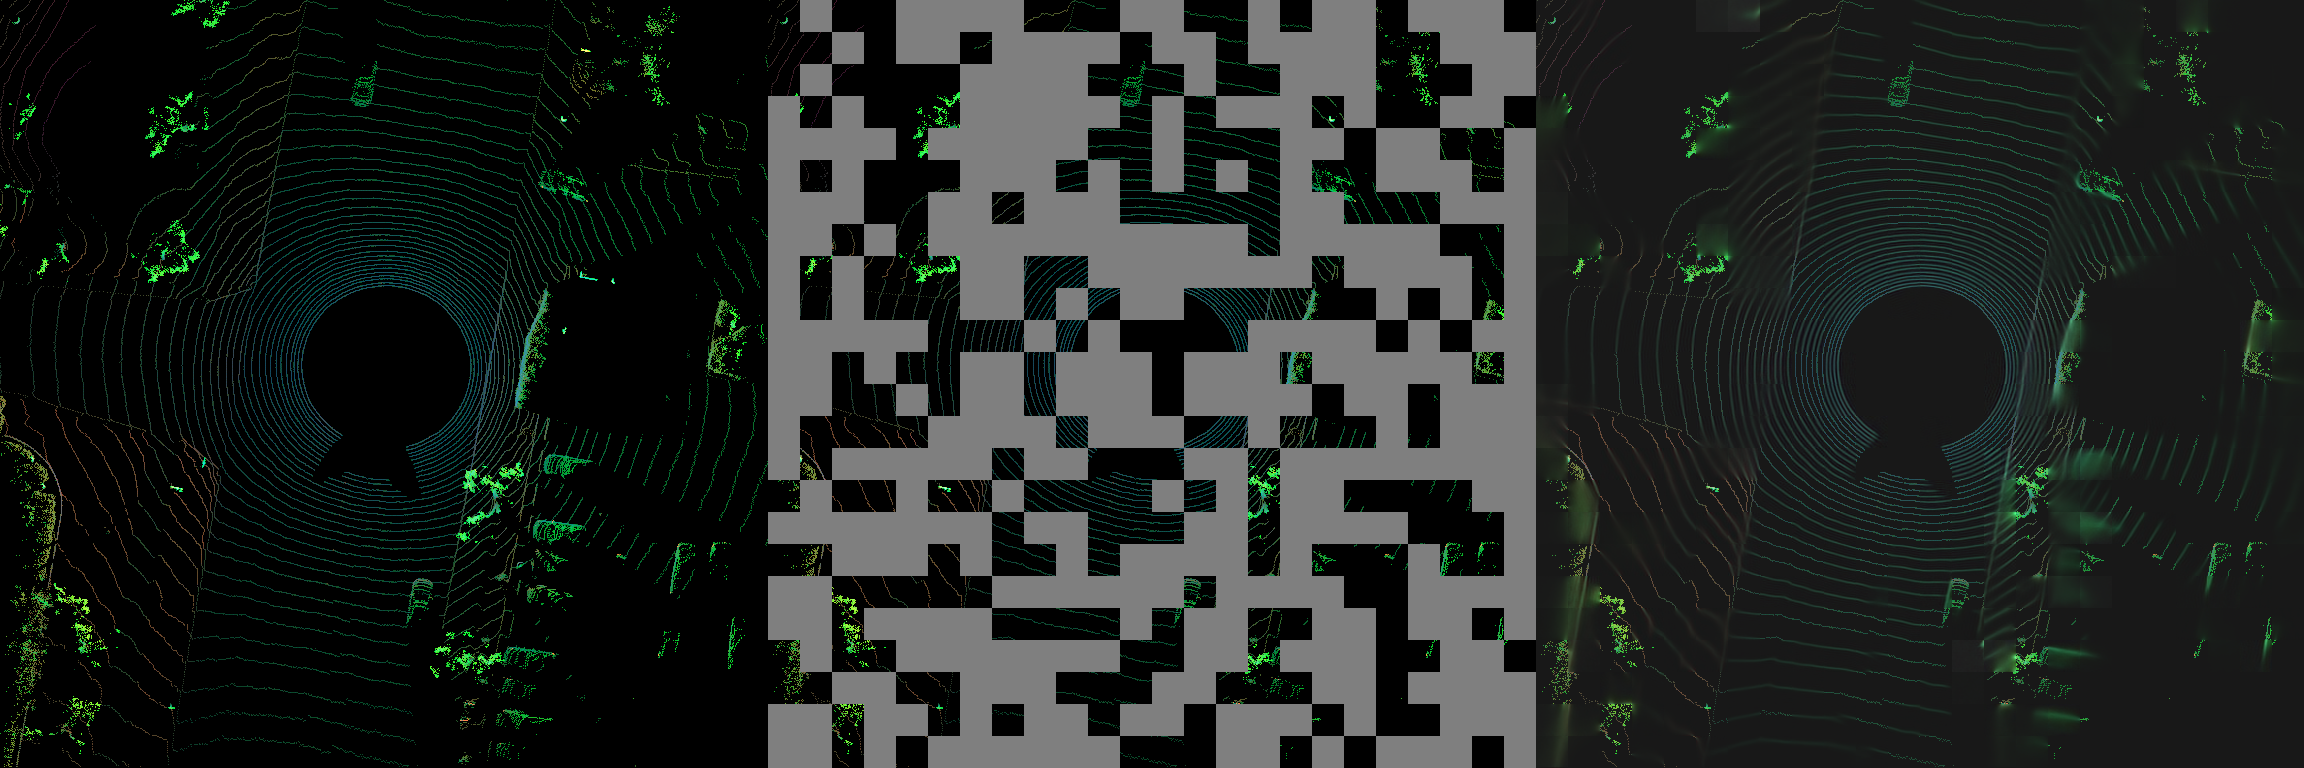
\includegraphics[width=420pt, angle=270]{pic/Hiera-Waymo.png}
\mainfont\fontsize{9pt}{9pt}\selectfont\caption{ \mainfont\fontsize{9pt}{9pt}\selectfont 3D Object Detection on Waymo Open using Hiera}
~\\[2mm]
\label{fig:mae_img}
\end{figure}
\begin{figure}[H]
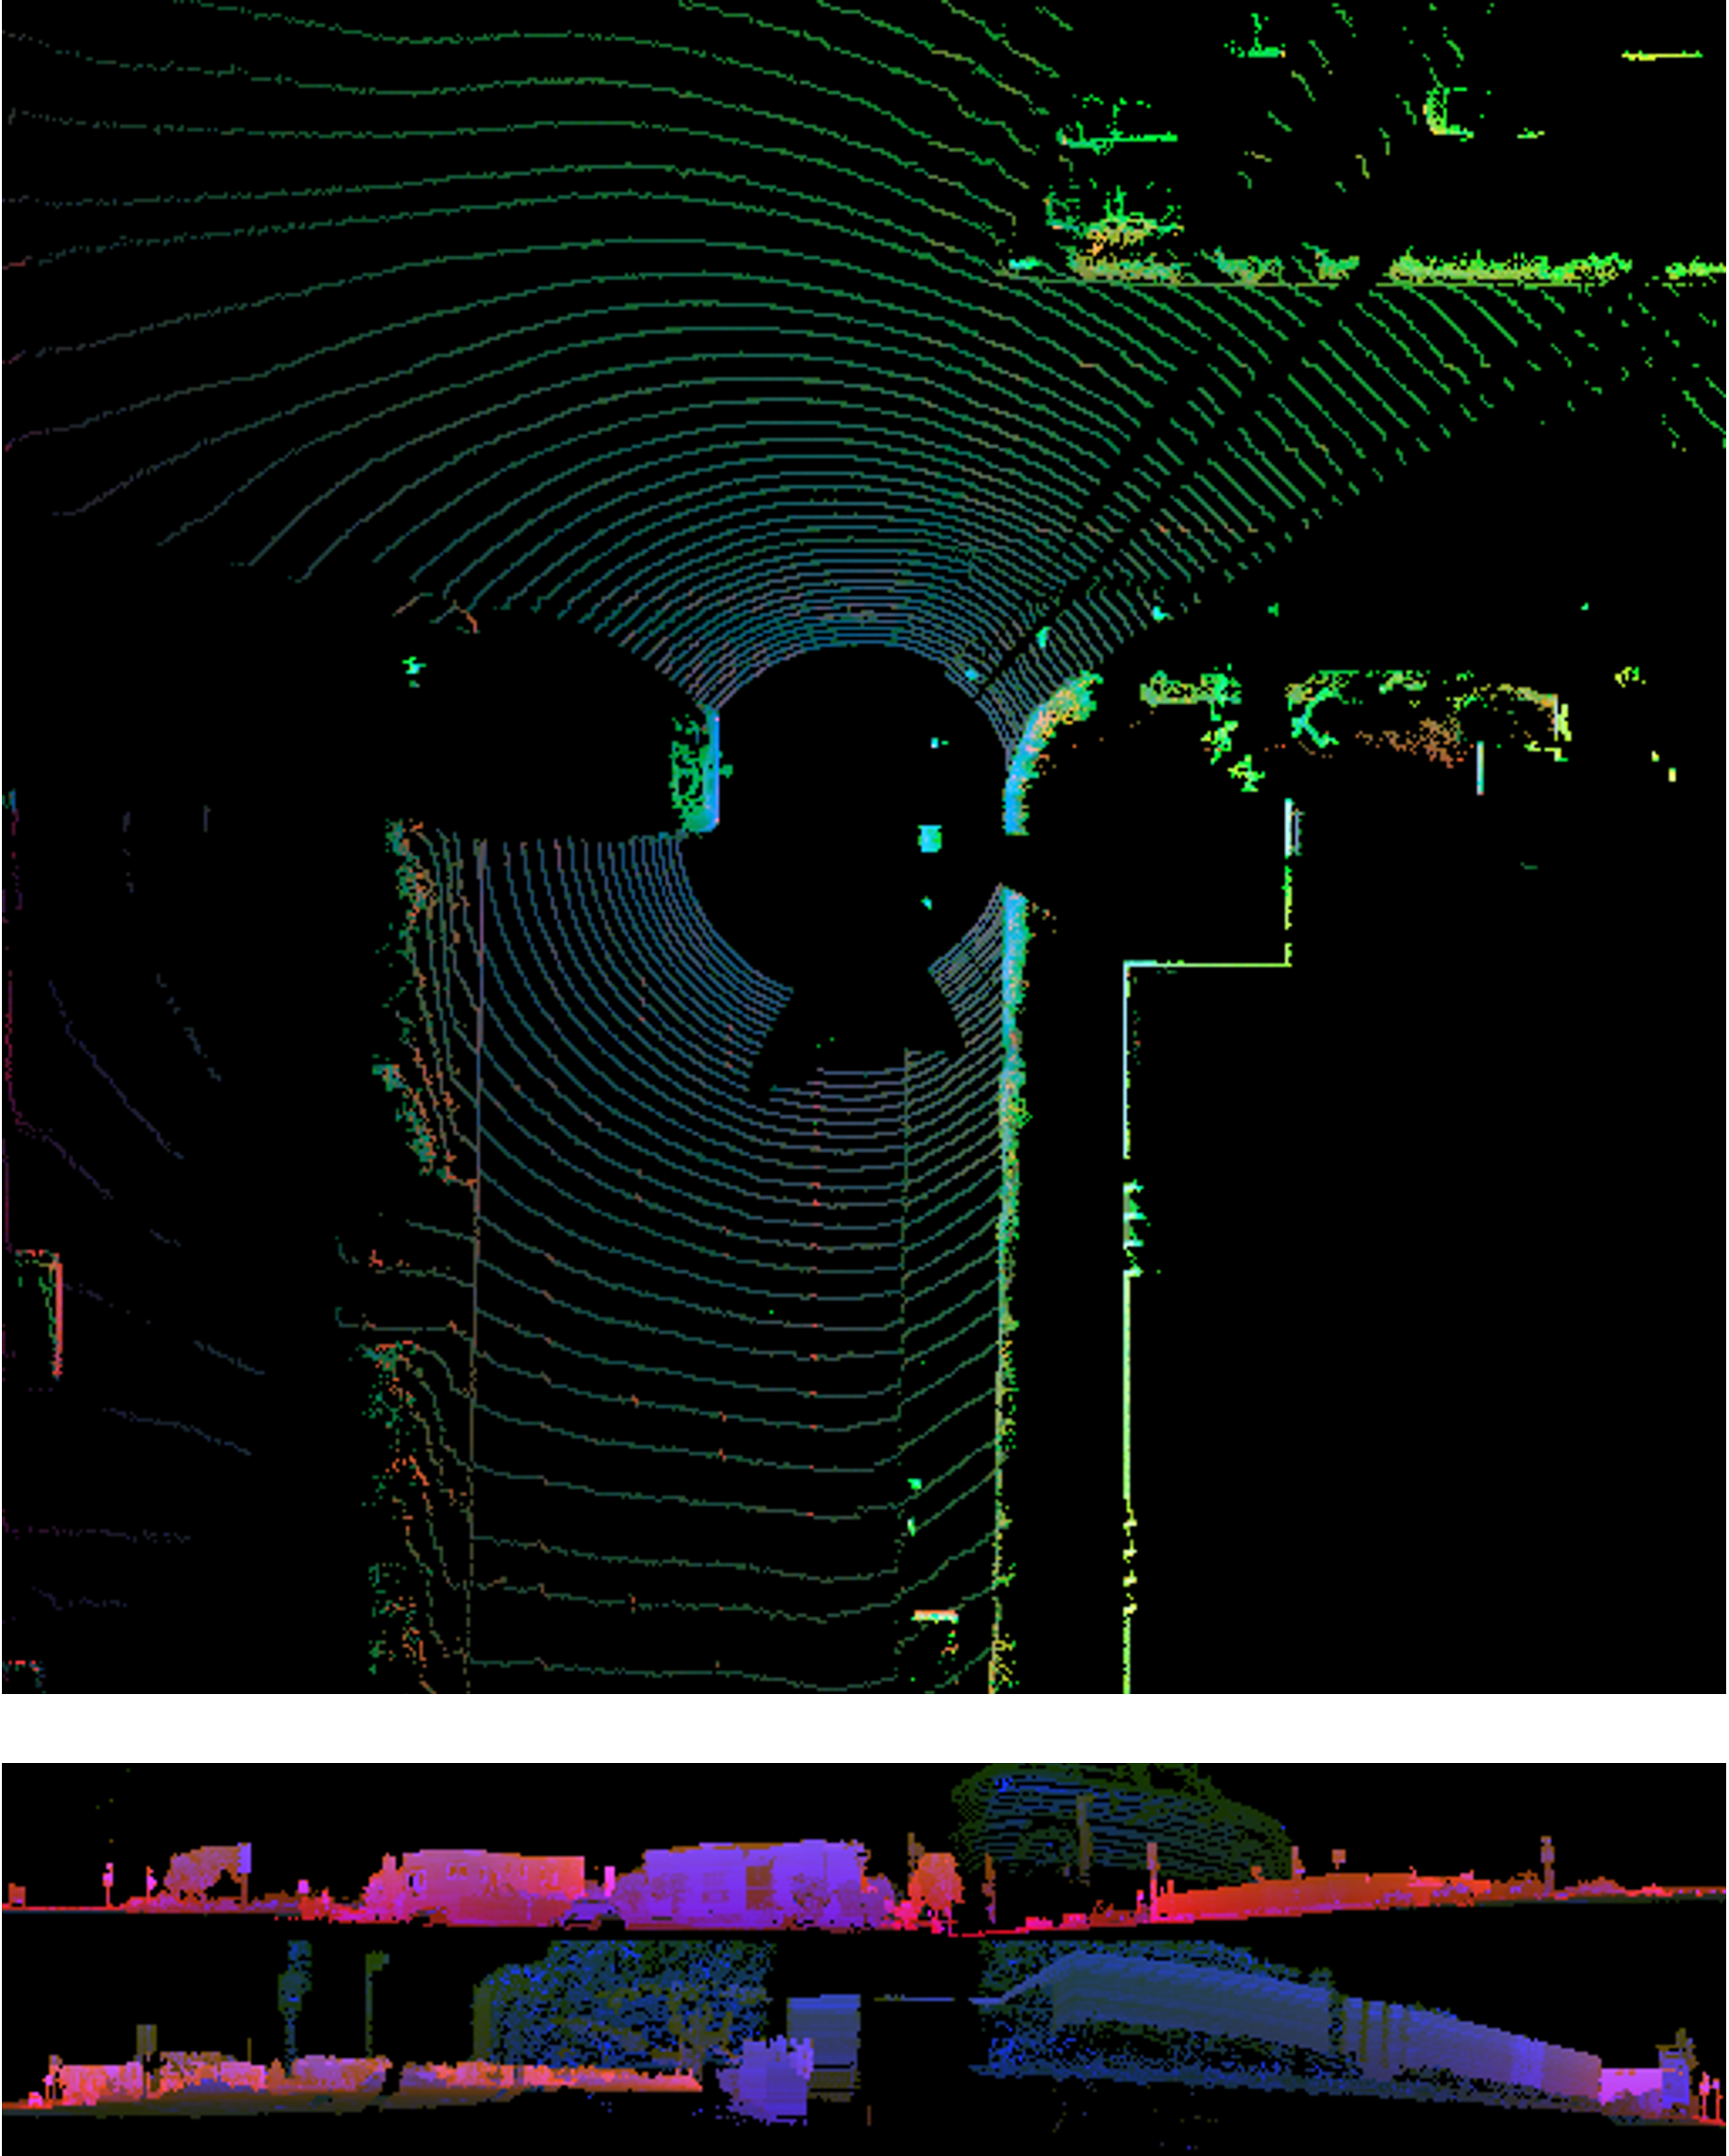
\includegraphics[width=140pt]{pic/fusion.png}
\mainfont\fontsize{9pt}{9pt}\selectfont\caption{ \mainfont\fontsize{9pt}{9pt}\selectfont3D Object Detection on Waymo Open using Hiera}
~\\[2mm]
\label{fig:fusion}
\end{figure}
\end{minipage}
\end{minipage}

